%%%%%%%%   Macro for the Two State Markov Chain Problems 
%%%%%%%%   The general solution here depends upon the 
%%%%%%%%   transition probabilities  p from A-> B and  q from B-> A . 
%%%%%%%%   You can set up one macro to generate this question.  
\newcounter{AtoB}  %  one digit from 1 to 9 
\newcounter{BtoA}  %  one digit from 1 to 9 
\newcounter{AtoA}  %  one digit from 1 to 9 
\newcounter{BtoB}  %  one digit from 1 to 9 
%%%%%%%%%%%%%%%%%%%%%%%%
%  Command for the markov Chain example.  Input two numbers from 1 to 9. 
%   For Example, call \TwoStateMarkov{3}{5}  
%%%%%%%%%%%%%%%%%%%%%%%% 
\newcommand{\TwoStateMarkov}[2]{
\setcounter{AtoB}{#1} \setcounter{BtoA}{#2} 
\setcounter{AtoA}{10-\theAtoB} \setcounter{BtoB}{10-\theBtoA} 
\question[2]
Calculate the steady state for the Markov chain shown below. Please show your work.  
        \begin{center}
        \begin{tikzpicture}[->,>=stealth',shorten >=1pt,auto,node distance=3cm,thick]
        \tikzstyle{every state}=[circle,fill=gray!10,draw,thick,,font=\bf, line width=0.4mm]
  %  
        \node[state] (A) {A};
        \node[state]  (B) [right of=A] {B};
        \path 
            (A) edge    [bend left] node {0.\theAtoB} (B)
                edge    [loop left] node {0.\theAtoA} (A)
            (B) edge    [loop right] node {0.\theBtoB} (B) 
                edge    [bend left] node {0.\theBtoA} (A);
        \end{tikzpicture} 
        \end{center}    
        
    \ifnum \Solutions=1 {\color{DarkBlue} \textit{Solutions.}         
        \begin{align}
            P-I &= \frac{1}{10} \begin{pmatrix} \theAtoA & \theBtoA \\ \theAtoB & \theBtoB\end{pmatrix} - \begin{pmatrix} 1&0\\0&1 \end{pmatrix} 
            \addtocounter{AtoA}{-10} \addtocounter{BtoB}{-10} 
            = \frac{1}{10} \begin{pmatrix} \theAtoA & \theBtoA \\ \theAtoB & \theBtoB\end{pmatrix}
            \sim \frac{1}{10} \begin{pmatrix}\theAtoA & \theBtoA \\0&0 \end{pmatrix}
        \end{align}
        The steady state is $ \frac1{\theAtoB+\theBtoA} \begin{pmatrix} \theBtoA \\ \theAtoB \end{pmatrix}$.
    }
    \else 
        \vfill
    \fi
}


\ifnum \Solutions=1 \newpage \fi


\ifnum \Version=0
    \question[2] If $x \in \mathbb R^2$ and $A = \begin{pmatrix} 5&-5\\5&5\end{pmatrix}$ then the transform $x \to Ax$ is the composition of a rotation and a scaling. Determine the angle of the rotation $\phi$ and the scale factor $r$. Assume that $\phi$ measures angles counter-clockwise from the $x_1$-axis. Please show your work. 
    
    \ifnum \Solutions=1 {\color{DarkBlue} \textit{Solutions.} 
    By inspection $A$ is a rotation-dilation matrix and therefore its eigenvalues are $\lambda = a \pm bi = 5 \pm 5i$.
    The scale factor is the distance $r = \sqrt{a^2 + b^2} = \sqrt{5^2 + 5^2} = 5\sqrt 2$, and the angle of rotation is $\tan^{-1} (b/a) = \pi/4$. 
    
    A few notes regarding the solution to this problem: 
    \begin{itemize}
        \item This is a \textit{show your work} question, so do write down some of your intermediate steps. 
        \item It isn't necessary to construct the characteristic polynomial and determine its roots to obtain these eigenvalues in this case, because the matrix $A$ is a rotation-dilation matrix. $2\times 2$ rotation dilation matrices always have $a\pm ib$ as their eigenvalues. For other problems where you need to compute eigenvalues, you should show some intermediate steps when computing eigenvalues. 
        \item One way to check whether your calculations for $r$ and $\phi$ are correct is to compute the output of the transform $x \ to Ax$ for a sample point. For example $Ae_1 = \begin{pmatrix} 5&-5\\5&5\end{pmatrix}\begin{pmatrix} 1\\0 \end{pmatrix} = \begin{pmatrix}5\\5 \end{pmatrix}$, which corresponds to the point $(5,5)$. The distance from the origin to this point is $5\sqrt2$ and the input point was rotated by $\pi/4$ radians counterclockwise to where it ended up after the transform. 
        \item It is ok to leave your answer for $\phi$ as $\phi = \tan^{-1} 1$. 
        \item If you would like to get more practice on a question like this, exercises from section 5.5 of our textbook are recommended. They might be in the MML Study Plan. 
    \end{itemize}
     
    
    

    } 
   \else
      
   \fi
\fi 


\ifnum \Version=1
    \question[2]  $A = \begin{pmatrix} 0&2\\2&3\end{pmatrix}$ has eigenvalues $\lambda_1 = 4$ and $\lambda_2 = -1$, with corresponding eigenvectors $v_1$ and $v_2$. Vector $p$ satisfies $p = \frac12 v_1 + 2v_2$. On the grids below, sketch a) the $\lambda_1$ and $\lambda_2$ eigenspaces, and b) the vector $Ap$. You do not need to show your work but please clearly label your eigenspaces. 
    \ifnum \Solutions=0
        \vspace{-12pt}
        \begin{center}
        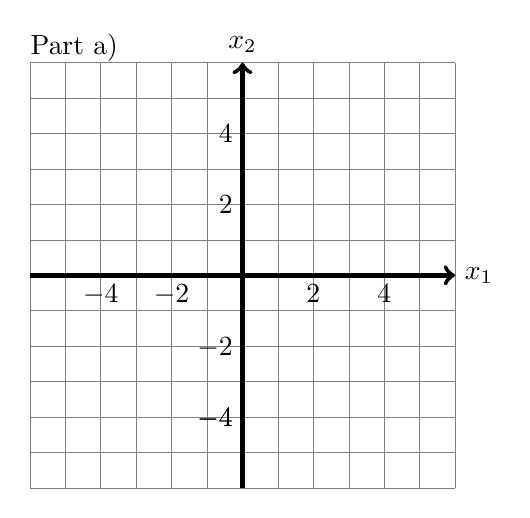
\begin{tikzpicture}[scale=.45]
        \draw[help lines, very thin, gray] (-6, -6) grid (6,6);
        \draw[ultra thick, ->] (-6, 0) -- (6, 0);
        \draw[ultra thick, ->] (0, -6) -- (0, 6);
        \node[overlay, above] at (-4.75, 5.75) { Part a)};
        \node[above] at (0, 6) {$x_2$};
        \node[right] at (6, 0) {$x_1$};
        \node[left] at (0, 2) {$2$};
        \node[below] at (2, 0) {$2$};
        \node[below] at (-2, 0) {$-2$};
        \node[left] at (0, -2.05) {$-2$};  
        \node[left] at (0, 4) {$4$};
        \node[below] at (4, 0) {$4$};
        \node[below] at (-4, 0) {$-4$};
        \node[left] at (0, -4.05) {$-4$};          
        \node[left] at (0, -4.05) {$-4$};          
        \end{tikzpicture}\qquad
        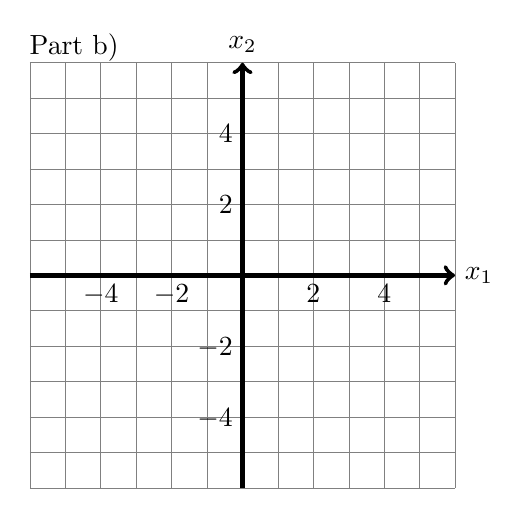
\begin{tikzpicture}[scale=.45]
        \draw[help lines, very thin, gray] (-6, -6) grid (6,6);
        \draw[ultra thick, ->] (-6, 0) -- (6, 0);
        \draw[ultra thick, ->] (0, -6) -- (0, 6);
        \node[overlay, above] at (-4.75, 5.75) { Part b) };
        \node[above] at (0, 6) {$x_2$};
        \node[right] at (6, 0) {$x_1$};
        \node[left] at (0, 2) {$2$};
        \node[below] at (2, 0) {$2$};
        \node[below] at (-2, 0) {$-2$};
        \node[left] at (0, -2.05) {$-2$};  
        \node[left] at (0, 4) {$4$};
        \node[below] at (4, 0) {$4$};
        \node[below] at (-4, 0) {$-4$};
        \node[left] at (0, -4.05) {$-4$};          
        \end{tikzpicture}
        \end{center}
        
        \vspace{24pt}
    \fi
    
    \ifnum \Solutions=1 {\color{DarkBlue} \textit{Solutions.} 
    \begin{enumerate}
        \item[a)] For eigenvalue $\lambda_1$: 
        \begin{align}
            A - \lambda_1 I = \begin{pmatrix} 4&2\\2&7 \end{pmatrix} - 4I = \begin{pmatrix} -4&2\\2&-1 \end{pmatrix}
        \end{align}
        A vector in the null space of this matrix is $v_1 = \begin{pmatrix} 1\\2\end{pmatrix}$. Any nonzero scalar multiple of this vector is also sufficient. For eigenvalue $\lambda_2$: 
        \begin{align}
            A - \lambda_2 I = \begin{pmatrix} 4&2\\2&7 \end{pmatrix}  + I = \begin{pmatrix} 1&2\\2&4 \end{pmatrix}
        \end{align}
        A vector in the null space of this matrix is $v_2 = \begin{pmatrix} -2\\1\end{pmatrix}$. Any nonzero scalar multiple of this vector is also sufficient. Sketching the spans of these vectors gives us the eigenspaces. Be sure to extend the lines to the edges of the graph, because eigenspaces are subspaces. 

        \begin{center}
        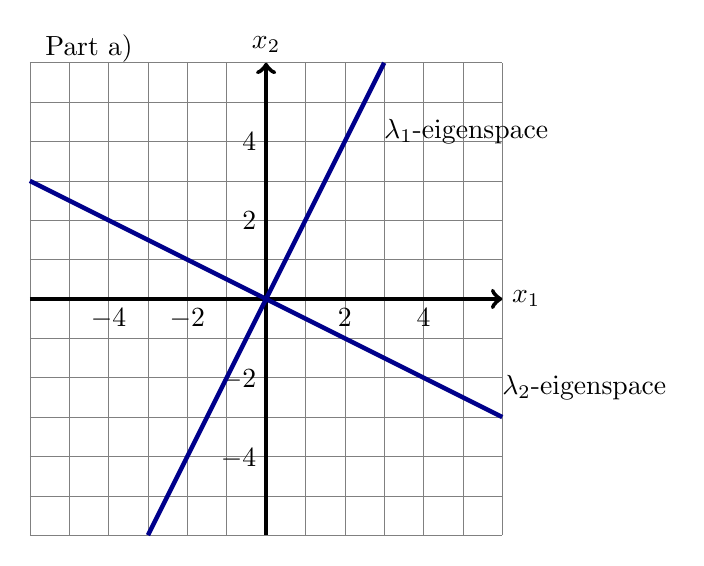
\begin{tikzpicture}[scale=.5]
        \draw[help lines, very thin, gray] (-6, -6) grid (6,6);
        \draw[ultra thick, ->] (-6, 0) -- (6, 0);
        \draw[ultra thick, ->] (0, -6) -- (0, 6);
        \node[overlay, above] at (-4.5, 5.75) {Part a)};
        \node[above] at (0, 6) {$x_2$};
        \node[right] at (6, 0) {$x_1$};
        \node[left] at (0, 2) {$2$};
        \node[below] at (2, 0) {$2$};
        \node[below] at (-2, 0) {$-2$};
        \node[left] at (0, -2.05) {$-2$};  
        \node[left] at (0, 4) {$4$};
        \node[below] at (4, 0) {$4$};
        \node[below] at (-4, 0) {$-4$};
        \node[left] at (0, -4.05) {$-4$};          
        \node[right] at (2.75,4.25) {$\lambda_1$-eigenspace};          
        \draw[ultra thick, DarkBlue,-] (-3, -6) -- (3, 6);
        \node[right] at (5.75,-2.25) {$\lambda_2$-eigenspace};          
        \draw[ultra thick, DarkBlue,-] (-6,3) -- (6,-3);        
        \end{tikzpicture}
        \end{center}
        For this particular matrix, the eigenspaces happen to be perpendicular to each other. Later in the course we will see why this is the case for this matrix. 

        \item[b)] We can approach this in a few different ways. One approach is to work out $p$ using the values of $v_1$ and $v_2$ from the previous part and then compute $Ap$: 
        \begin{align}
            Ap = A (\frac12 v_1 + 2v_2) = \begin{pmatrix} 0&2\\2&3\end{pmatrix}\left( \frac12 \begin{pmatrix} 1\\2 \end{pmatrix} +2 \begin{pmatrix} -2\\1\end{pmatrix}\right) = \begin{pmatrix} 0&2\\2&3\end{pmatrix}\begin{pmatrix} -7/2\\ 3\end{pmatrix} = \begin{pmatrix} 6\\2\end{pmatrix}
        \end{align}
        
        Or, using $Av = \lambda v$ we have that 
        \begin{align}
            Ap = A(\frac12 v_1 + 2v_2) 
            = \frac12 Av_1  + 2Av_2 
            = \frac 12 \lambda_1v_1 + 2\lambda_2v_2 
            = 2\begin{pmatrix} 1\\2 \end{pmatrix} - 2\begin{pmatrix} -2\\1 \end{pmatrix} 
            = \begin{pmatrix} 6\\2\end{pmatrix}
        \end{align}
        The vector $Ap = \begin{pmatrix} 6\\2\end{pmatrix}$ is sketched below. 
            \begin{center}
            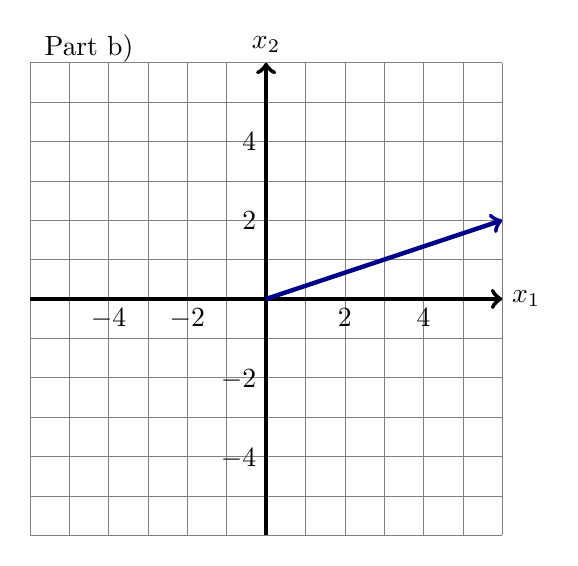
\begin{tikzpicture}[scale=.5]
            \draw[help lines, very thin, gray] (-6, -6) grid (6,6);
            \draw[ultra thick, ->] (-6, 0) -- (6, 0);
            \draw[ultra thick, ->] (0, -6) -- (0, 6);
            \node[overlay, above] at (-4.5, 5.75) {Part b)};
            \node[above] at (0, 6) {$x_2$};
            \node[right] at (6, 0) {$x_1$};
            \node[left] at (0, 2) {$2$};
            \node[below] at (2, 0) {$2$};
            \node[below] at (-2, 0) {$-2$};
            \node[left] at (0, -2.05) {$-2$};  
            \node[left] at (0, 4) {$4$};
            \node[below] at (4, 0) {$4$};
            \node[below] at (-4, 0) {$-4$};
            \node[left] at (0, -4.05) {$-4$};          
            \draw[ultra thick, DarkBlue,->] (0,0) -- (6,2);     
            \end{tikzpicture}
            \end{center}
    \end{enumerate}        
    } 

   \else
      
   \fi
\fi 



\ifnum \Version=2
    \ifnum \Solutions=1 \newpage \fi 
    
    \question[2] The $2\times 2$ matrix $A$ has eigenvalues $\lambda_1=-1$ and $\lambda_2=2$, with eigenspaces indicated in the picture. Vectors $x$ and $y$ are also shown below. Draw $A x$ and $A y$.

    \begin{center}
    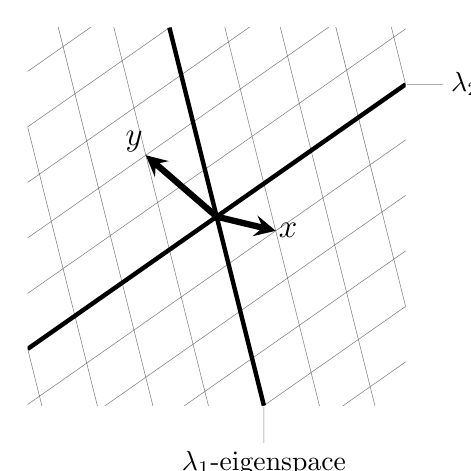
\begin{tikzpicture}[scale=.6,vectorB/.style={-stealth, black, thick, line width=0.8mm}]

      \begin{scope}
      \clip (-4, -4) rectangle (4, 4);
      \begin{scope}[cm={1,2.8/4,1/4,-1,(0,0)}]
        \draw[help lines] (-6, -6) grid (6, 6);
        \draw[vectorB] (0, 0) -- (1, 1) node[right, inner sep=0] {\large $ x$};
        \draw[vectorB] (0, 0) -- (-1, -2) node[above left, inner sep=0] {\large $ y$};
      \end{scope}
      \draw[ultra thick] (-4, -2.8) -- (4, 2.8);
      \draw[ultra thick] (-1, 4) -- (1, -4);
      \node[circle, inner sep=.4mm, fill] at (0, 0) {};
      \end{scope}
      \node[pin={[overlay, inner sep=1mm]0:{$\lambda_2$-eigenspace}}, outer sep=0, inner sep=0] at (4, 2.8) {};
      \node[pin={[overlay, inner sep=1mm]270:{$\lambda_1$-eigenspace}}, outer sep=0, inner sep=0] at (1, -4) {};
    \end{tikzpicture}
    \end{center}    
    
    \ifnum \Solutions=0
        \vspace{12pt}
    \fi

    \ifnum \Solutions=1
        {\color{DarkBlue} 
            \textbf{Solutions}\\
            Take $v_1$ to be any non-zero vector in the $\lambda_1$ eigenspace, and $v_2$ to be any non-zero vector in the $\lambda_2$-eigenspace. We could for example make the following choices for $v_1$ and $v_2$. }
            \begin{center}
            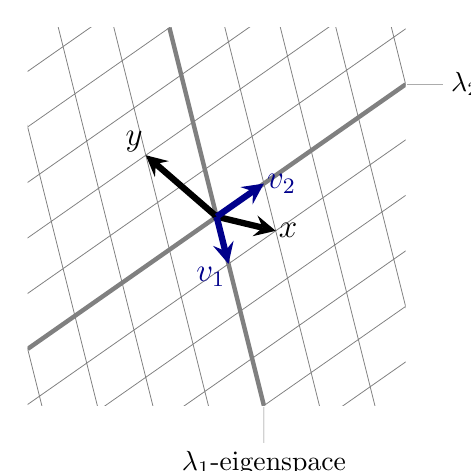
\begin{tikzpicture}[scale=.6,vectorB/.style={-stealth, black, thick, line width=0.8mm},vectorR/.style={-stealth, DarkBlue, thick, line width=0.8mm}]
                \begin{scope}
                    \clip (-4, -4) rectangle (4, 4);
                    \draw[gray,ultra thick] (-4, -2.8) -- (4, 2.8);
                    \draw[gray, ultra thick] (-1, 4) -- (1, -4);
                    \node[circle, inner sep=.4mm, fill] at (0, 0) {};              
                    \begin{scope}[cm={1,2.8/4,1/4,-1,(0,0)}]
                        \draw[help lines,line width=0.1mm] (-6, -6) grid (6, 6);
                        \draw[vectorB] (0, 0) -- (1, 1) node[right, inner sep=0] {\large $ x$};
                        \draw[vectorB] (0, 0) -- (-1, -2) node[above left, inner sep=0] {\large $ y$};
                        \draw[vectorR] (0, 0) -- (0,1) node[below left, inner sep=0] {\large $ v_1$};
                        \draw[vectorR] (0, 0) -- (1, 0) node[right, inner sep=0] {\large $ v_2$};
                    \end{scope}
                \end{scope}
                \node[pin={[overlay, inner sep=1mm]0:{$\lambda_2$-eigenspace}}, outer sep=0, inner sep=0] at (4, 2.8) {};
                \node[pin={[overlay, inner sep=1mm]270:{$\lambda_1$-eigenspace}}, outer sep=0, inner sep=0] at (1, -4) {};
            \end{tikzpicture}
            \end{center}    
            {\color{DarkBlue} 
            With this choice we have $x = v_1 + v_2$, and $y = -2v_1 - v_2$. We want to sketch $A\vec x$ and $A\vec y$, but:
            \begin{align}
                A x &= A(v_1 + v_2) = Av_1 + A v_2 = \lambda_1v_1 + \lambda_2v_2 = -v_1 + 2v_2 \\
                A y &= A(-2v_1 - v_2) = -2Av_1 - A v_2 = -2\lambda_1v_1 - \lambda_2v_2 = 2v_1 - 2v_2 
            \end{align}
            So we need to sketch $Ax = -v_1 + 2v_2$ and $Ay = 2v_1 - 2 v_2$. They are sketched below.}
            \begin{center}
            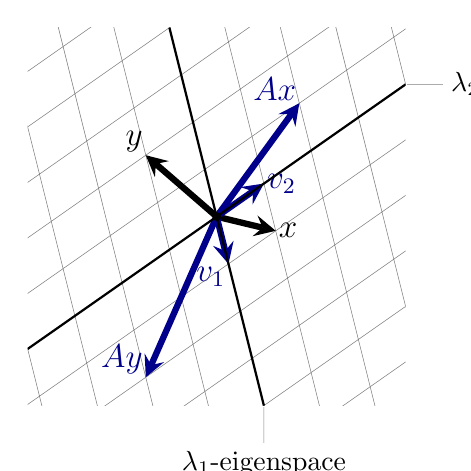
\begin{tikzpicture}[scale=.6,vectorB/.style={-stealth, black, thick, line width=0.8mm},vectorR/.style={-stealth, DarkBlue, thick, line width=0.8mm}]
              \begin{scope}
              \clip (-4, -4) rectangle (4, 4);
              \begin{scope}[cm={1,2.8/4,1/4,-1,(0,0)}]
                \draw[help lines] (-6, -6) grid (6, 6);
                \draw[vectorB] (0, 0) -- (1, 1) node[right, inner sep=0] {\large $ x$};
                \draw[vectorB] (0, 0) -- (-1, -2) node[above left, inner sep=0] {\large $ y$};
                \draw[vectorR] (0, 0) -- (0,1) node[below left, inner sep=0] {\large $ v_1$};
                \draw[vectorR] (0, 0) -- (1, 0) node[right, inner sep=0] {\large $ v_2$};                
                \draw[vectorR] (0, 0) -- (2,-1) node[above left, inner sep=0] {\large $ Ax$};
                \draw[vectorR] (0, 0) -- (-2,2) node[above left, inner sep=0] {\large $ Ay$};
              \end{scope}
              \draw[ thick] (-4, -2.8) -- (4, 2.8);
              \draw[ thick] (-1, 4) -- (1, -4);
              \node[circle, inner sep=.4mm, fill] at (0, 0) {};
              \end{scope}
              \node[pin={[overlay, inner sep=1mm]0:{$\lambda_2$-eigenspace}}, outer sep=0, inner sep=0] at (4, 2.8) {};
              \node[pin={[overlay, inner sep=1mm]270:{$\lambda_1$-eigenspace}}, outer sep=0, inner sep=0] at (1, -4) {};
            \end{tikzpicture}
            \end{center}

    \fi
\fi




\ifnum \Version=3
    \question[2] Calculate the steady state for the Markov chain shown below. Please show your work.  
        \begin{center}
        \begin{tikzpicture}[->,>=stealth',shorten >=1pt,auto,node distance=3cm,thick]
        \tikzstyle{every state}=[circle,fill=gray!10,draw,thick,,font=\bf, line width=0.4mm]
    
        \node[state] (A) {A};
        \node[state]  (B) [right of=A] {B};
        \path 
            (A) edge    [bend left] node {0.3} (B)
                edge    [loop left] node {0.7} (A)
            (B) edge    [loop right] node {0.4} (B) 
                edge    [bend left] node {0.6} (A);
        \end{tikzpicture} 
        \end{center}    

    \ifnum \Solutions=1 {\color{DarkBlue} \textit{Solutions.} 
    
        \begin{align}
            P-I &= \frac{1}{10} \begin{pmatrix} 7 & 6 \\ 3 & 4\end{pmatrix} - \begin{pmatrix} 1&0\\0&1 \end{pmatrix} = \frac{1}{10}\begin{pmatrix}-3&6\\3&-6 \end{pmatrix} \sim \begin{pmatrix}-1&2\\0&0 \end{pmatrix}
        \end{align}
        The steady-state is: 
        $$ \vec q = \frac{1}{3}\begin{pmatrix}2\\1 \end{pmatrix}$$
        } 
    \fi
\fi

\ifnum \Version=4
    \question[2] Calculate the steady state for the Markov chain shown below. Please show your work.  
        \begin{center}
        \begin{tikzpicture}[->,>=stealth',shorten >=1pt,auto,node distance=3cm,thick]
        \tikzstyle{every state}=[circle,fill=gray!10,draw,thick,,font=\bf, line width=0.4mm]
    
        \node[state] (A) {A};
        \node[state]  (B) [right of=A] {B};
        \path 
            (A) edge    [bend left] node {0.3} (B)
                edge    [loop left] node {0.7} (A)
            (B) edge    [loop right] node {0.8} (B) 
                edge    [bend left] node {0.2} (A);
        \end{tikzpicture} 
        \end{center}    

    \ifnum \Solutions=1 {\color{DarkBlue} \textit{Solutions.} 
    
        \begin{align}
            P-I &= \frac{1}{10} \begin{pmatrix} 7 & 2 \\ 3 & 8\end{pmatrix} - \begin{pmatrix} 1&0\\0&1 \end{pmatrix} = \frac{1}{10}\begin{pmatrix}-3&2\\3&-2 \end{pmatrix} \sim \begin{pmatrix}-3&2\\0&0 \end{pmatrix}
        \end{align}
        The steady-state is: 
        $$ \vec q = \frac{1}{5}\begin{pmatrix}2\\3 \end{pmatrix}$$
        } 
    \else
    \vfill         
    \fi
\fi


\ifnum \Version=5
    \question[2] Calculate the steady state for the Markov chain shown below. Please show your work.  
        \begin{center}
        \begin{tikzpicture}[->,>=stealth',shorten >=1pt,auto,node distance=3cm,thick]
        \tikzstyle{every state}=[circle,fill=gray!10,draw,thick,,font=\bf, line width=0.4mm]
    
        \node[state] (A) {A};
        \node[state]  (B) [right of=A] {B};
        \path 
            (A) edge    [bend left] node {0.3} (B)
                edge    [loop left] node {0.7} (A)
            (B) edge    [loop right] node {0.8} (B) 
                edge    [bend left] node {0.2} (A);
        \end{tikzpicture} 
        \end{center}    

    \ifnum \Solutions=1 {\color{DarkBlue} \textit{Solutions.} 
    
        \begin{align}
            P-I &= \frac{1}{10} \begin{pmatrix} 7 & 2 \\ 3 & 8\end{pmatrix} - \begin{pmatrix} 1&0\\0&1 \end{pmatrix} = \frac{1}{10}\begin{pmatrix}-3&2\\3&-2 \end{pmatrix} \sim \begin{pmatrix}-3&2\\0&0 \end{pmatrix}
        \end{align}
        The steady-state is: 
        $$ \vec q = \frac{1}{5}\begin{pmatrix}2\\3 \end{pmatrix}$$
        } 

    \fi
\fi


\ifnum \Version=6
  \TwoStateMarkov{4}{7}
\fi    

\ifnum \Version=7
    \TwoStateMarkov{7}{3} 
\fi

\ifnum \Version=8
    \TwoStateMarkov{7}{5}
\fi      



\ifnum \Version=12 % NOT NEEDED? 
    \question[2] Calculate the steady state for the Markov chain shown below. Please show your work.  
        \begin{center}
        \begin{tikzpicture}[->,>=stealth',shorten >=1pt,auto,node distance=3cm,thick]
        \tikzstyle{every state}=[circle,fill=gray!10,draw,thick,,font=\bf, line width=0.4mm]
    
        \node[state] (A) {A};
        \node[state]  (B) [right of=A] {B};
        \path 
            (A) edge    [bend left] node {0.3} (B)
                edge    [loop left] node {0.7} (A)
            (B) edge    [loop right] node {0.4} (B) 
                edge    [bend left] node {0.6} (A);
        \end{tikzpicture} 
        \end{center}    

    \ifnum \Solutions=1 {\color{DarkBlue} \textit{Solutions.} 
      Find the probability vector in the kernel of $P_I$. 
        \begin{align}
            P-I &= \frac{1}{10} \begin{pmatrix} 7 & 6 \\ 3 & 4\end{pmatrix} - \begin{pmatrix} 1&0\\0&1 \end{pmatrix} = \frac{1}{10}\begin{pmatrix}-3&6\\3&-6 \end{pmatrix} \sim \begin{pmatrix}-1&2\\0&0 \end{pmatrix}
        \end{align}
        The steady-state is: 
        $$ \vec q = \frac{1}{3}\begin{pmatrix}2\\1 \end{pmatrix}$$
        } 
    \else 
        \vfill
    \fi
\fi



\ifnum \Version=13 % NOT NEEDED? 
    \question[2] Calculate the steady state for the Markov chain shown below. Please show your work.  
        \begin{center}
        \begin{tikzpicture}[->,>=stealth',shorten >=1pt,auto,node distance=3cm,thick]
        \tikzstyle{every state}=[circle,fill=gray!10,draw,thick,,font=\bf, line width=0.4mm]
    
        \node[state] (A) {A};
        \node[state]  (B) [right of=A] {B};
        \path 
            (A) edge    [bend left] node {0.2} (B)
                edge    [loop left] node {0.8} (A)
            (B) edge    [loop right] node {0.4} (B) 
                edge    [bend left] node {0.6} (A);
        \end{tikzpicture} 
        \end{center}    

    \ifnum \Solutions=1 {\color{DarkBlue} \textit{Solutions.} 
    
        The steady state has eigenvalue 1. So it is the probability vector in the null space (i.e. - the kernel) of $P-I$. 
        \begin{align} 
            P-I &= \frac{1}{10} \begin{pmatrix} 8 & 6 \\ 2 & 4\end{pmatrix} - \begin{pmatrix} 1&0\\0&1 \end{pmatrix} = \frac{1}{10}\begin{pmatrix}-2&6\\2&-6 \end{pmatrix} \sim \begin{pmatrix}-1&3\\0&0 \end{pmatrix}
        \end{align}
        The steady-state is: 
        $$ \vec q = \frac{1}{4}\begin{pmatrix}3\\1 \end{pmatrix}$$
        } 
    \fi
\fi